\pagestyle{fancy}
\headheight 20pt
\lhead{Ph.D. Thesis --- R. Woods}
\rhead{McMaster - Physics \& Astronomy}
\chead{}
\lfoot{}
\cfoot{\thepage}
\rfoot{}
\renewcommand{\headrulewidth}{0.1pt}
\renewcommand{\footrulewidth}{0.1pt}


\chapter{Code Tests}
\label{chap:codetests}
\thispagestyle{fancy}

In this chapter, I present a variety of tests to demonstrate the strengths and limitations of the above algorithm. Many test cases have been drawn from previous RT papers including \citet{ilievEt06,gendelevKrumholz12,skinnerOstriker13}. This chapter also include tests of accuracy and scaling of the algorithm.

\section{Single Star Field}
\label{sec:glass}

In the first test, we demonstrate the most basic functionality of the code: the ability to create a simple radiation field from a single star. In the optically thin limit, the flux should fall off as $1/r^2$,

\begin{equation}
\label{eq:r2flux}
F = \frac{L}{4\pi r^2},
\end{equation}

Where L is the luminosity of the star, set to 1 (in code units) in this case. We initialize 64$^3$ gas particles in a ``glass'' by creating a grid of particles and allowing them to settle with repulsive forces and periodic boundary conditions. This gives a roughly homogeneous density throughout the cube. The positions in x, y, and z range from -0.5 to 0.5 in code units. In the case with absorption, particles are given an opacity and density such that $\rho\kappa = 1$. Thus,  optical depth just just equal to radius and is one across the length of the box. The analytic solution is

\begin{equation}
\label{eq:thickflux}
F = \frac{L}{4\pi r^2} \exp{-r}.
\end{equation}

In both runs, SPH density estimates are done, but no forces (hydrodynamic, gravitational, or otherwise) are present. Figure \ref{fig:singlestarflux} shows flux vs radius for the two cases.

\begin{figure}
        \centering
        \begin{subfigure}[b]{0.45\textwidth}
                \includegraphics[width=\textwidth]{graphics/placeholder.eps}
                \caption{No Absorption}
                \label{fig:singlestarthin}
        \end{subfigure}
        ~ 
        \begin{subfigure}[b]{0.45\textwidth}
                \includegraphics[width=\textwidth]{graphics/placeholder.eps}
                \caption{$\tau$ = 1.}
                \label{fig:singlestarthick}
        \end{subfigure}
        \caption[Flux for a single star]{Flux vs radius for a single star in a) the case of no absorption and b) the case with an optical depth of 1 across the box.}
        \label{fig:singlestarflux}
\end{figure}

In the first case, our answer is accurate to machine precision since all interactions are exact (the center of luminosity of a cell is the exact location of the star for a single source). In the second case, there is slight variance in the answer due to the fact that the density field is not exactly homogeneous. This is shown in figure \ref{fig:fluxdensityvariance}.

\begin{figure}
        \centering
        \begin{subfigure}[b]{0.45\textwidth}
                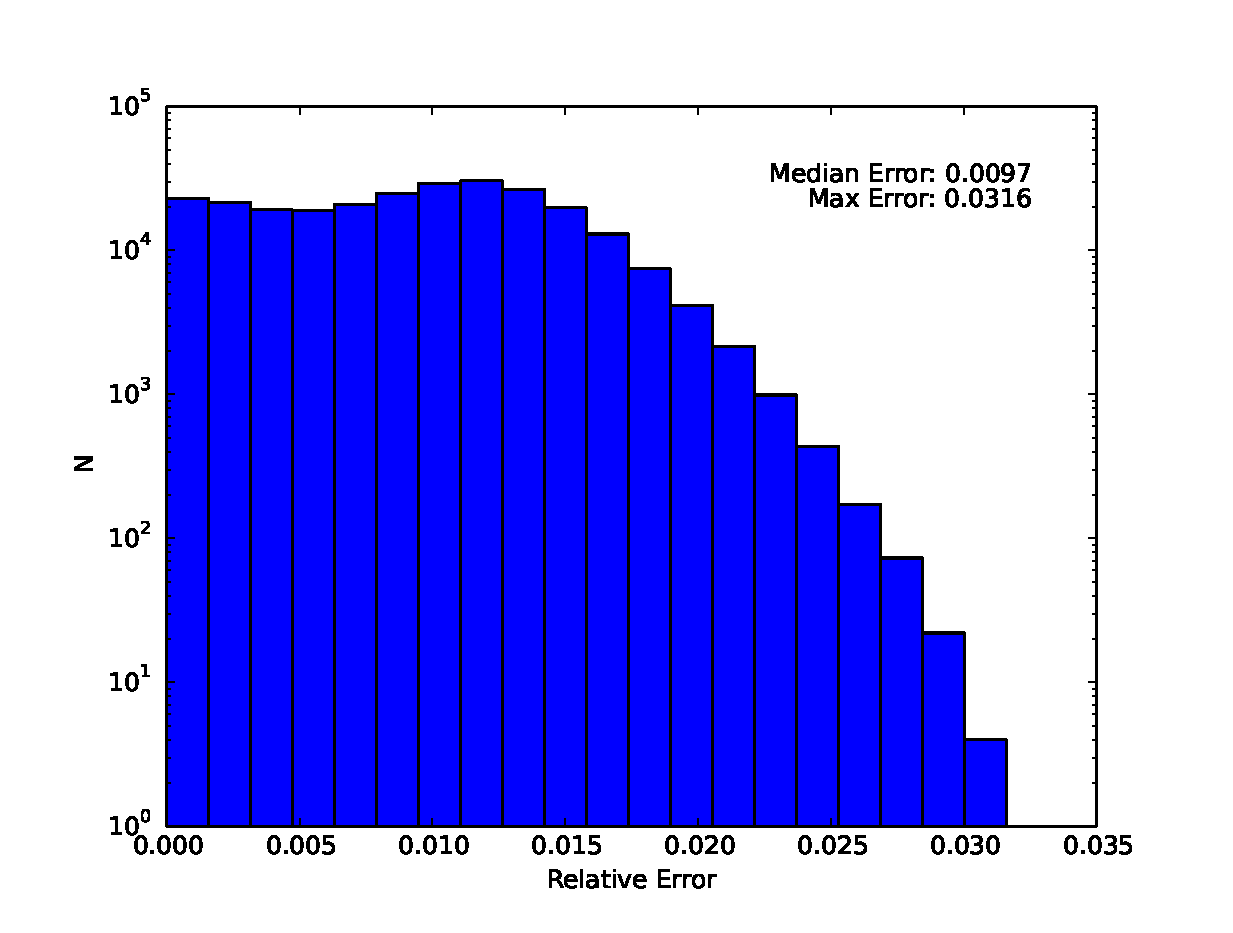
\includegraphics[width=\textwidth]{graphics/errorNorm.eps}
                \caption{Error distribution of flux with SPH density estimate [log x axis, normalize y].}
                \label{fig:fluxerrorsingle}
        \end{subfigure}
        ~ 
        \begin{subfigure}[b]{0.45\textwidth}
                \includegraphics[width=\textwidth]{graphics/errorOp.eps}
                \caption{Variance in SPH density [log x axis, normalize y].}
                \label{fig:optimization}
        \end{subfigure}
        \caption[Absolute flux error distribution and SPH density variance.]{Figure a) shows the distribution of absolute error in fluxes that particles receive, which is shown to be attributed to b) the variance in the SPH density estimate as compared to the average.}
        \label{fig:fluxdensityvariance}
\end{figure}

In figure \ref{fig:fluxerrorsingle}, the error is entirely associated with the variance in SPH density. If particles are set by hand to be an exact density, we are accurate to machine precision, as should be the case. Figure \ref{fig:optimization} shows the effect of an optimization used in the code. Instead of doing the tree climb to the receiving leaf once for each particle in the leaf, we do it once for the entire leaf to the center of mass. As is seen, this introduces only a few percent error in the flux and so is acceptable.

\section{Effects of Averaging the Source}
\label{sec:averagingsource}

We now look closely at what effects averaging sources can have on results. To demonstrate this, we use the same glass of particles from section \ref{sec:glass}, but insert two sources slightly offset from one another at locations p1 = (0.15, 0.25, 0.25) and p2 = (0.35, 0.25, 0.25) in code units. This means their average position is at $\bar{p}$=(0.25, 0.25, 0.25).

\begin{figure}
        \centering
        \begin{subfigure}[b]{0.45\textwidth}
                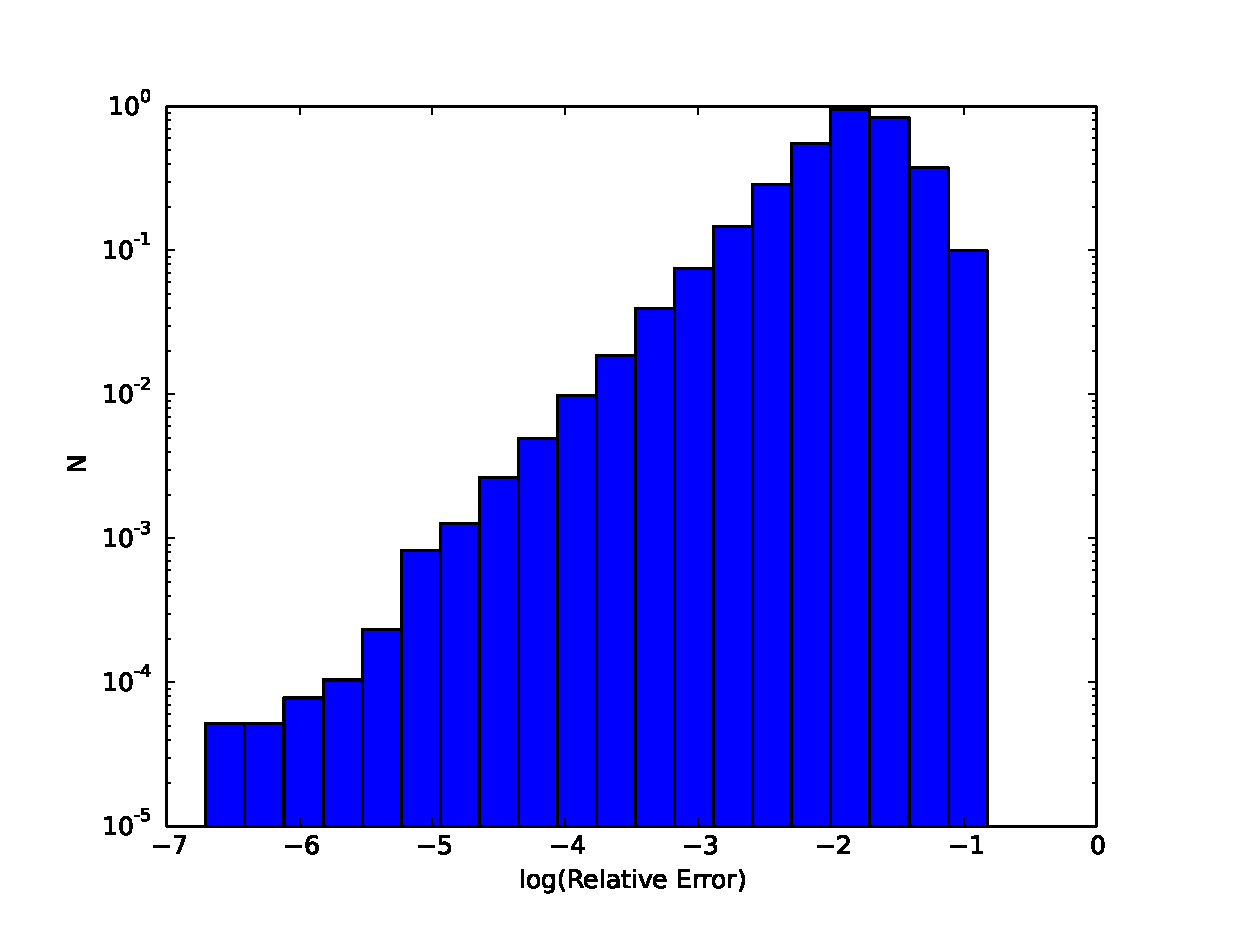
\includegraphics[width=\textwidth]{graphics/error2star.eps}
                \caption{Error distribution of flux}
                \label{fig:2starerrordist}
        \end{subfigure}
        ~ 
        \begin{subfigure}[b]{0.45\textwidth}
                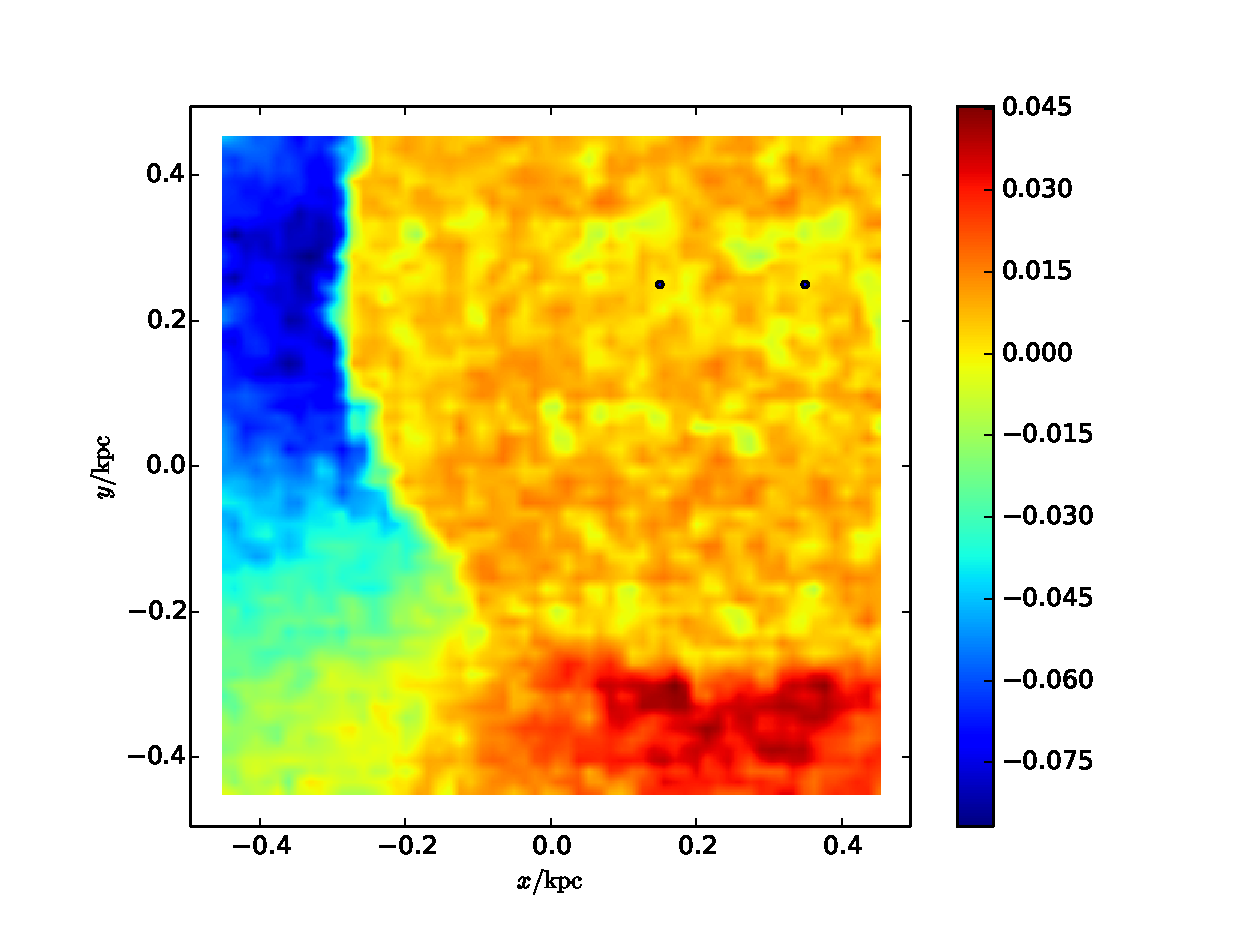
\includegraphics[width=\textwidth]{graphics/error2starMap.eps}
                \caption{Map of error}
                \label{fig:2starerrormap}
        \end{subfigure}
        \caption[Flux error for two star configuration]{Figure a) shows the distribution of errors for two stars, while figure b) shows a map of error vs position (color = error, slice in the z plane).}
        \label{fig:2starerror}
\end{figure}

Figure \ref{fig:2starerrormap} shows that the largest errors occur along the axis that the stars lie on, where flux is systematically underestimated. Errors also occur perpendicular to the axis of the stars, where flux is overestimated. The reason for this is simple if one considers the geometry. Since absorption is proportional to the exponent of radius (see equation \ref{eq:thickflux}), then the average diminishment to the flux is

\begin{equation}
\label{eq:averageofdim}
f = \frac{e^{-r_1}+e^{-r_2}}{2},
\end{equation}

\noindent
which is greater than

\begin{equation}
\label{eq:dimofaverage}
f = e^{-(r_1+r_2)/2} = e^{-r_1/2}e^{-r_2/2}
\end{equation}

\noindent
for [some values] and less than equation \ref{eq:dimofaverage} for [some values]. A larger diminishment means a smaller flux, so flux is underestimated. While 15\% seems like a significant error, we note that less than 1\% of particles have errors more than 10\%, and less than 10\% of particles have errors larger than 5\%. As well, compared to many of the assumptions that need to be made in a physical simulation (see chapter \ref{chap:galaxyformation}), 15\% is not unreasonable.

\section{Timings and Scaling}
\label{sec:timing}

We have tested the scaling of the code with the number of sources present in the simulation. We start with a glass of 64$^3$ gas particles, and add N$_{source}$ star particles to the initial condition by evenly distributing the source particles throughout the volume. In distributing the source particles evenly, we create the most stressful conditions possible for the code. This is due to the fact that if the star particles are distributed evenly, the minimal amount of source merging occurs. Were the sources clustered, most leaf nodes would only interact with a single merged cell. For this reason, the scaling and timing should be seen as an upper bound. Simulations are run multiple times per source for a single time step, and the run times per source are averaged together. As well, we run each simulation with refinement turned off, and with refinement set to be on at all times (this is a worst case scenario). The simulations were carried out in serial.

\begin{figure}
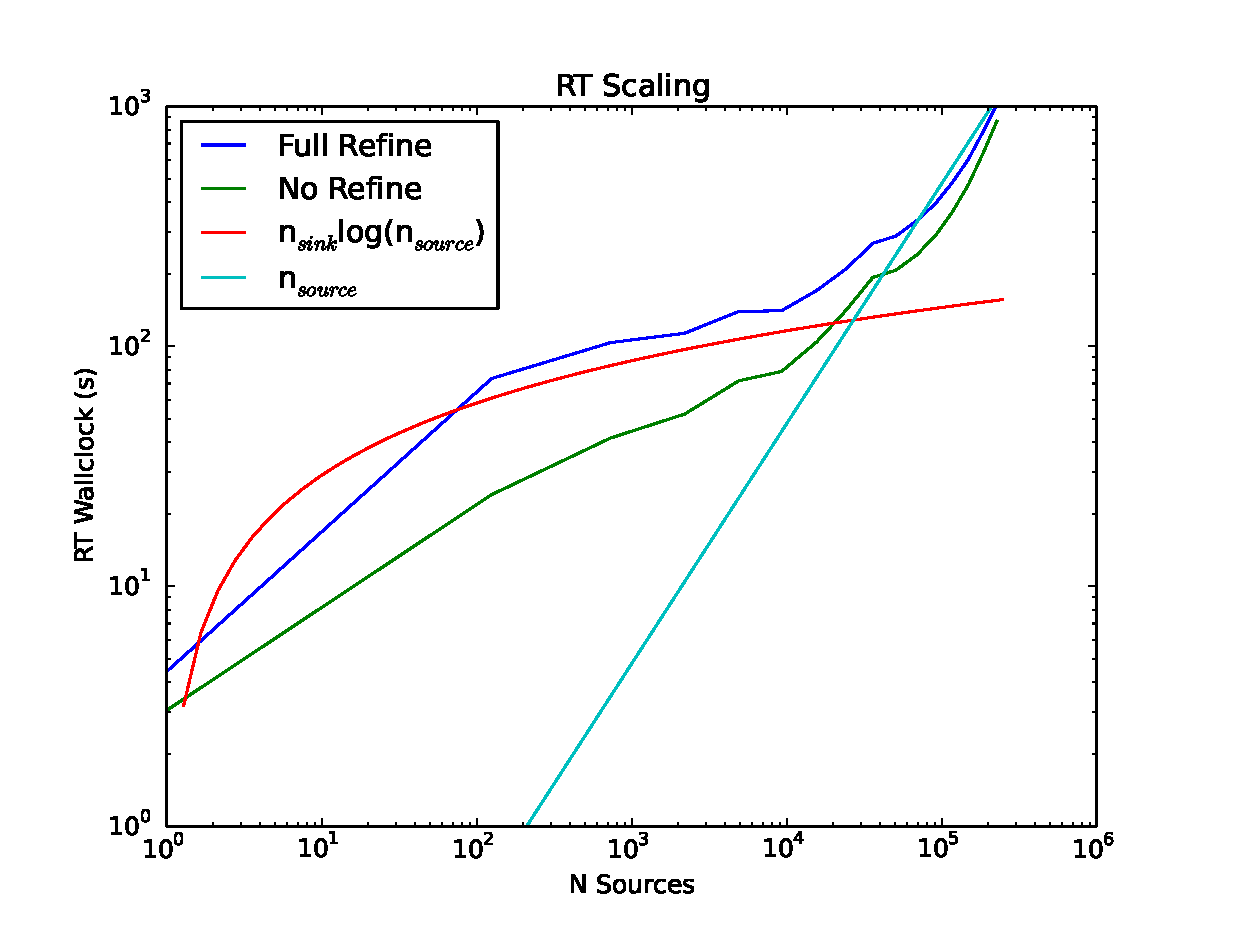
\includegraphics[width=\textwidth]{graphics/timings.eps}
\caption[Wall time vs the number of sources.]{Wall time vs the number of sources.}
\label{fig:scaling}
\end{figure}

Figure \ref{fig:scaling} shows that at lower numbers of sources, scaling goes as roughly log($N_{source}$), as was suggested in chapter \ref{chap:method}. However, as the number of sources approaches the number of sinks, and because the sources are evenly distributed, the ray tracing cost (discussed in section \ref{sec:resolvingleaves}) begins to dominate and the algorithm scales as $N_{source}$. We note that this scenario is quite unlikely in most astrophysical simulations, where star formation is very often clustered. It is therefore not a scenario we expect to run into often.

It is also important to note the effect of refinement. At small numbers of sources, full refinement incurs only a small cost of roughly 20\%. At high numbers of sources, the ray trace has already become the dominant cost, and so refinement adds only about 10\% additional computing time. However, the intermediate region, around 100 sources, refinement can increase computing time by up to a factor of four. Again, this is a worst case scenario as we have set the code to refine at all times, independent of cell properties.

%In terms of realistic costs, we present an isolated galaxy disk in chapter \ref{chap:galaxyformation.} Simulations of the isolated disk contained roughly 10$^5$ gas particles and 10$^5$ star particles, and our algorithm caused the total walltime of the simulation to increase by a factor of roughly [Ask James]. Note that part of this additional cost is extra cooling and heating integration in the cooling code.

\section{The Str\"omgren Sphere}
\label{sec:stromgren}

The str\"omgren sphere is a theoretical ionized sphere of gas. It was first discussed by Bengt Str\"omgren in 1938 \citep{stromgren39}. We start with a cloud of homogeneous neutral Hydrogen gas and an ionizing source, commonly representing an O or B-type star, at the center. As the photons from the source ionize the hydrogen, the optical depth of the gas decreases, and so the ionizing photons move further out creating an ionization front. As the front moves out, the photon density as a function of radius falls off simply due to $1/r^2$ geometry and eventually a point is reached where the ionization rate falls to the recombination rate. At this point, the front stops and reaches equilibrium.

%One can solve for this radius by setting the photon density as a function of radius to the recombination rate and solving for radius \citep{stromgren39,spitzer78},
%
%\begin{equation}
%\label{eq:stromgrenradius}
%R_S = \left( \frac{3}{4\pi} \frac{\dot{N_{\gamma}}}{\alpha n_H^2}\right).
%\end{equation}
%
%One can also find the growth rate of the front,
%
%\begin{equation}
%\label{eq:stromgrentime}
%R(t) = R_S[1-\exp{(t/t_{\mbox{recomb}})}]^{1/3}.
%\end{equation}
%
%The above equations are the solutions for the evolution of a sharp ionization front, meaning that we have assumed the transition from ionized to neutral is infinitesimal in size. In order to solve for a non-sharp front, we must solve some equations numerically. FILL IN METHOD HERE.

\subsection{The Isothermal Case}
\label{sec:isostromgren}

In the simplest case, the ionizing source is assumed to emit photons at exactly 13.7 ev, meaning that the hydrogen gas is ionized but not heated. Cooling is also disabled, meaning that the gas is isothermal. If we assume that the ionization front propagates until the ionization rate drops to equal the recombination rate of the ambient medium, then we can solve for the equilibrium ionization radius by setting the two rates equal. This gives (e.g. \citep{tielens05})

%\begin{equation}
%\label{eq:fluxrecomb}
%F = \int_0^{r_s} n_e n_H \alpha_B(T) dl,
%\end{equation}
%
%where $n_e$ is the number density of electrons, $n_H$ is the number density of neutral Hydrogen, $\alpha_B$ is the case B recombination coefficient for Hydrogen for a given temperature, and $r_s$ is the equilibrium radius or ``Str\"omgren radius.'' 

\begin{equation}
\label{eq:strmogrenradius}
R_S = \left( \frac{3}{4\pi} \frac{\dot{N_{\gamma}}}{\alpha n_H^2}\right),
\end{equation}

\noindent
where $\dot{N_{\gamma}}$ is the source luminosity in photons per second, $\alpha$ is the recombination rate, and $n_H^2$ is the Hydrogen number density. One can also solve for the radius as a function of time \citep{spitzer78},

\begin{equation}
\label{eq:stromgrentime}
R(t) = R_S[1-\exp{(t/t_{\mbox{recomb}})}]^{1/3},
\end{equation}

\noindent
where $t_{\mbox{recomb}}$ is the recombination time of the gas. The above derivation assumes a ``sharp'' ionization front, meaning the transition from ionized to neutral is across an infinitesimal region. In practice, the transition region is small compared to the size of the ionized region, but there is structure interior to the Str\"omgren radius that is not accounted for by simply solving for the equilibrium radius. In order to solve for a non-sharp ionization front, we must numerically integrate the Hydrogen ionization equations and the flux equation with absorption (eqaution \ref{eq:thickflux}) \citep{osterbrockFerland2006}. In the following tests, we include both the sharp and non-sharp ionization front solutions for comparison to our results.

We follow the initial conditions of \citet{ilievEt06}; the medium is initially neutral with a temperature 1e5 K and a density of 1e-3 cm$^{-3}$. An ionizing source is turned on at t = 0 that emits $\dot{N} = 5e48$ photons s$^{-1}$ at 13.6 ev. We use a cross section $\sigma = 6.3e-18$ cm$^2$ and a recombination rate of $\alpha = 2.59e-13$ cm$^{-3}$ s$^{-1}$, typical of 1e5 K gas. These values give a Str\"omgren radius of 5.38 kpc and a recombination time (1/$n_H \alpha$) of 125 Myr.

\begin{figure}
        \centering
        \begin{subfigure}[b]{0.45\textwidth}
                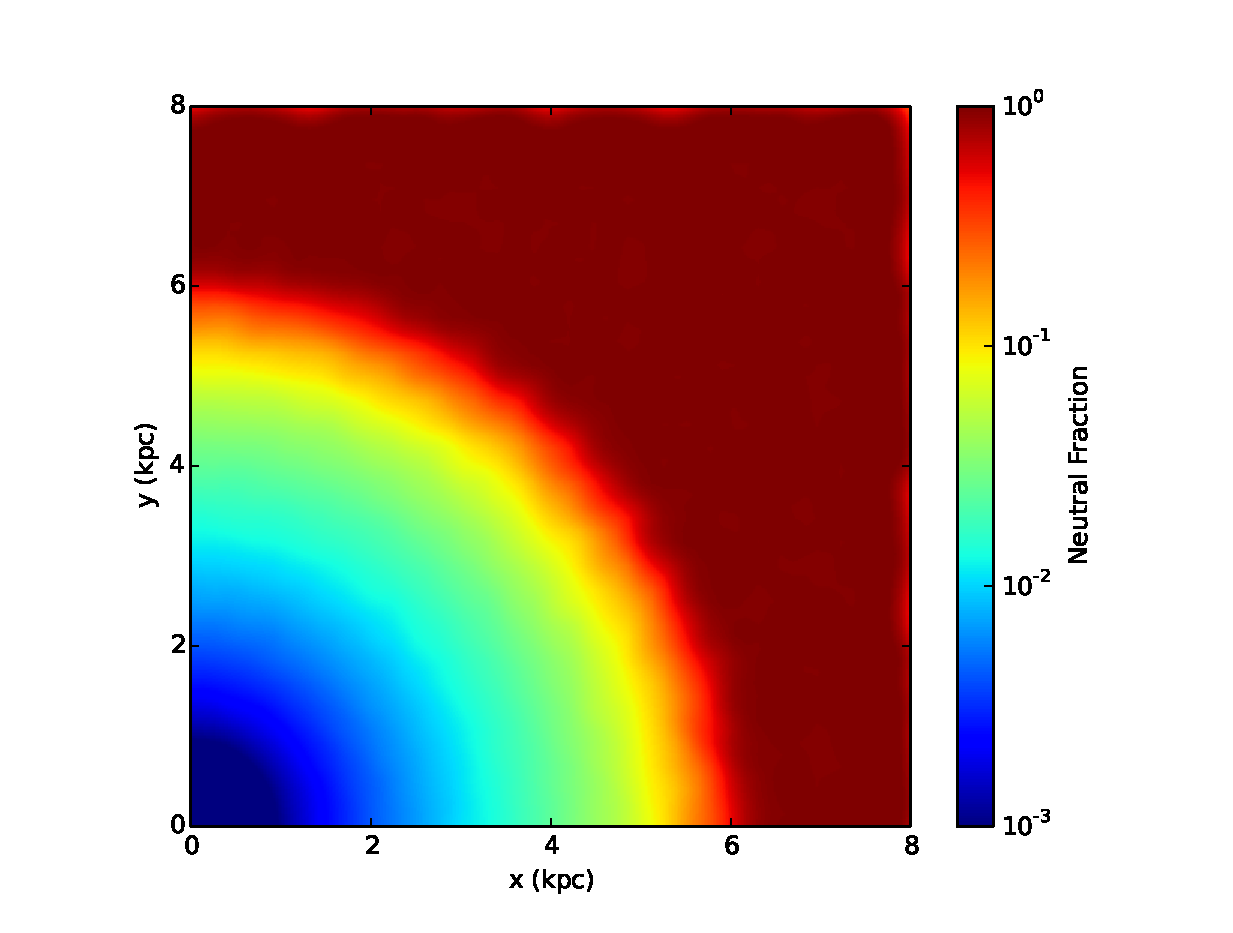
\includegraphics[width=\textwidth]{graphics/ifront6401000slice.eps}
                \caption{}
                \label{fig:stromgrenisoslice}
        \end{subfigure}
        ~
        \begin{subfigure}[b]{0.45\textwidth}
                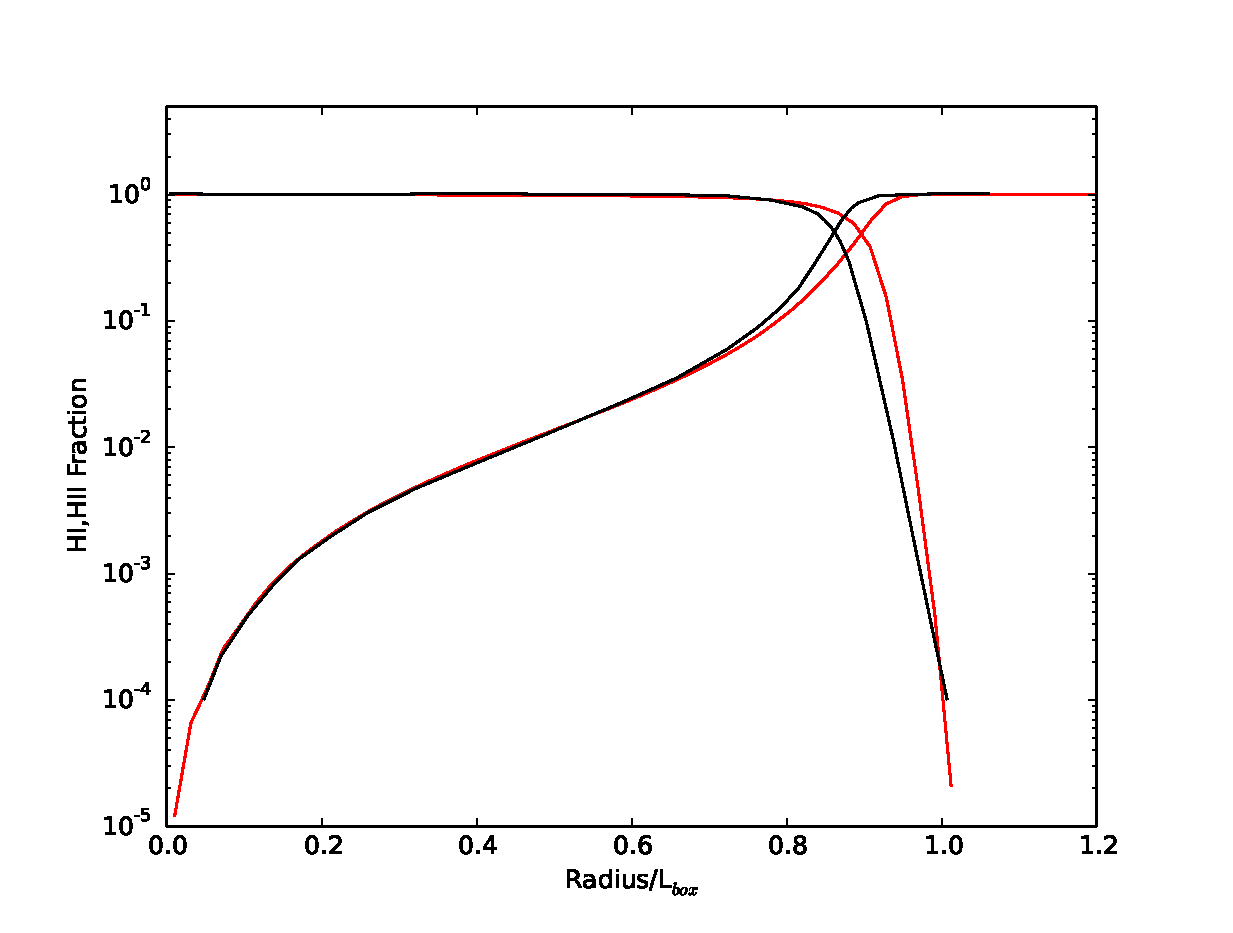
\includegraphics[width=\textwidth]{graphics/ifront6401000HI.eps}
                \caption{}
                \label{fig:stromgrenisoHI}
        \end{subfigure}
		\\        
        \begin{subfigure}[b]{0.45\textwidth}
                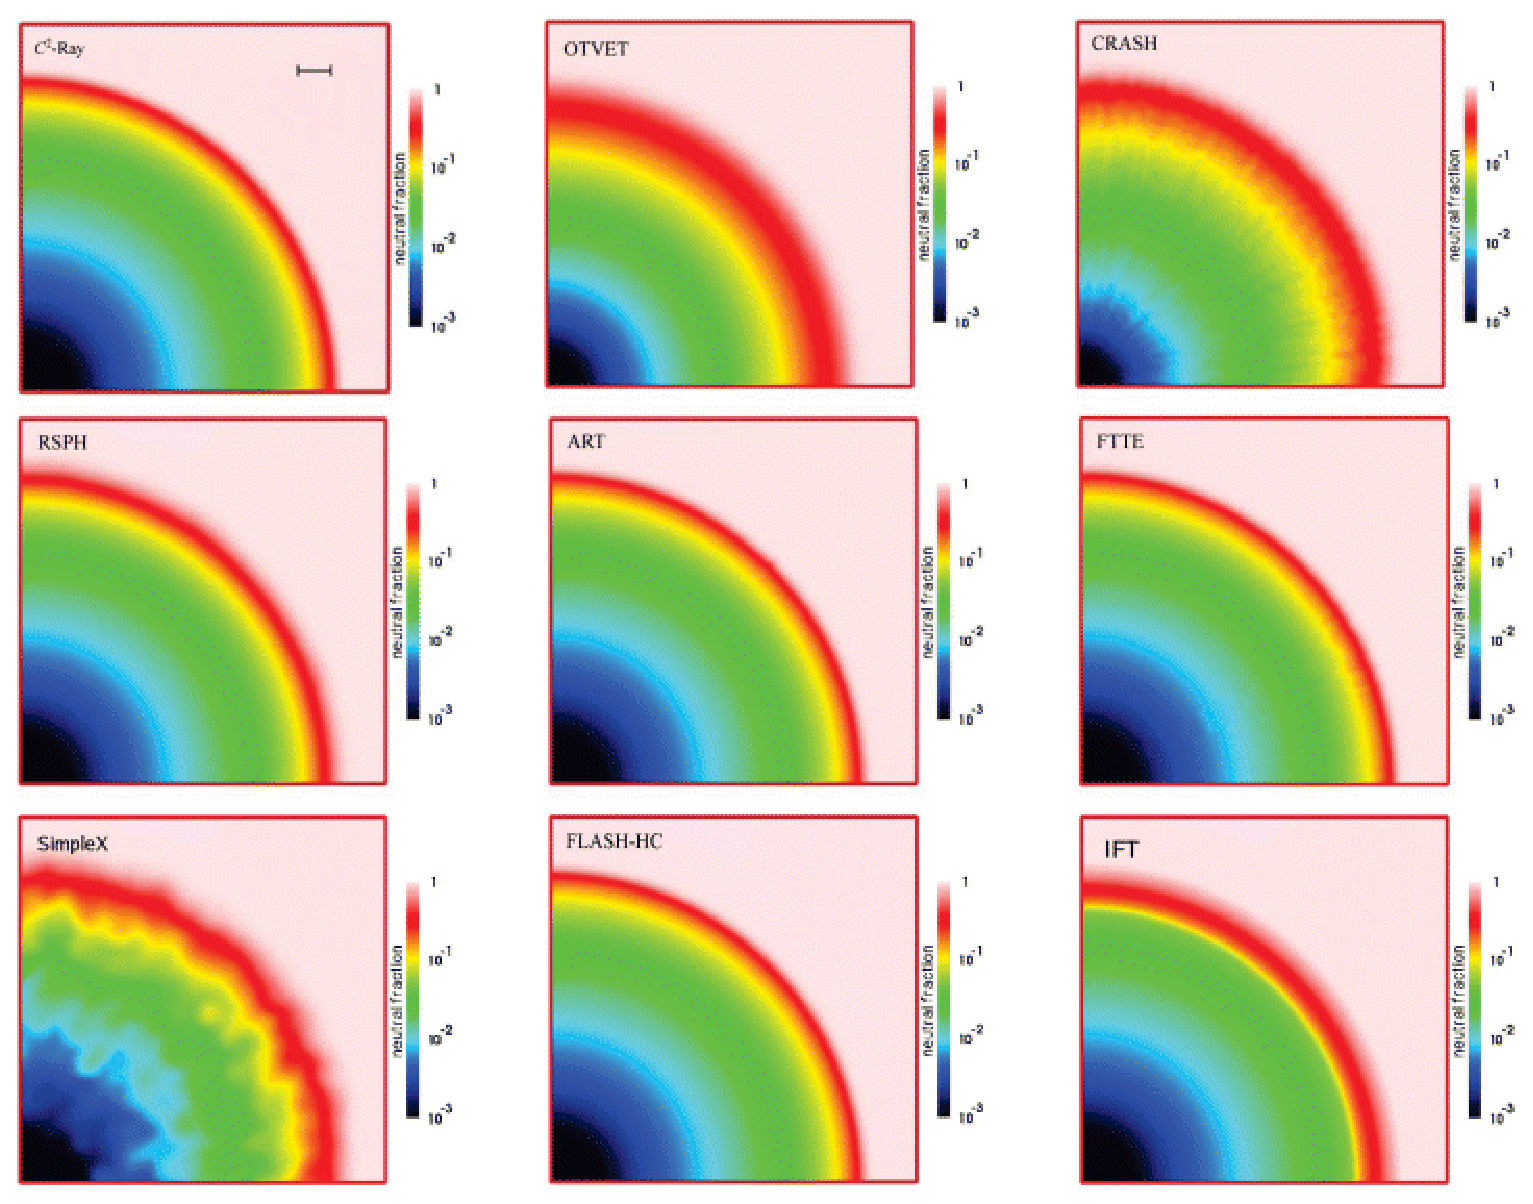
\includegraphics[width=\textwidth]{graphics/iliev06f6.eps}
                \caption{}
                \label{fig:ilievEtf6}
        \end{subfigure}
        ~
        \begin{subfigure}[b]{0.45\textwidth}
                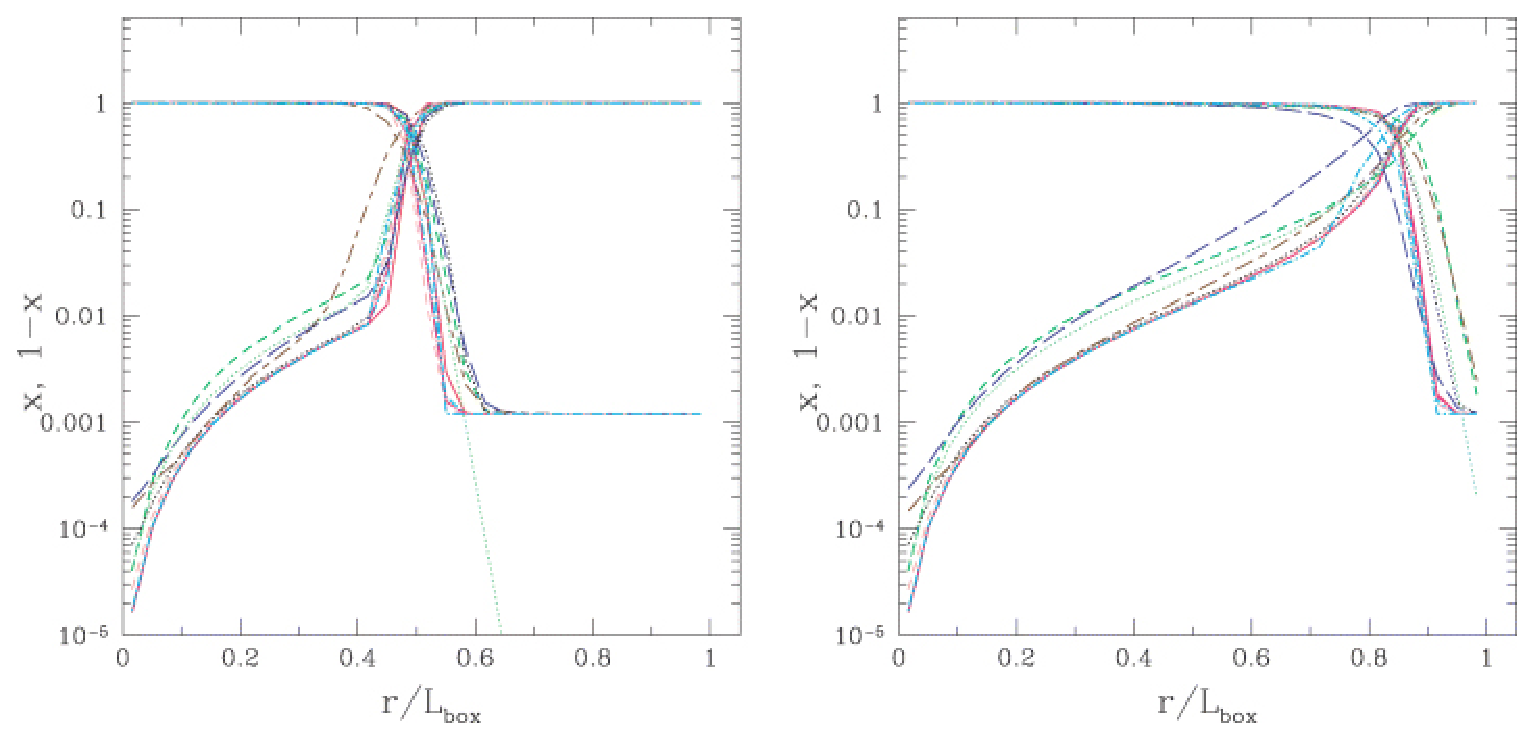
\includegraphics[width=\textwidth]{graphics/iliev06f8.eps}
                \caption{}
                \label{fig:ilievEtf8}
        \end{subfigure}
        \caption[The isothermal Str\"omgren Sphere.]{Figure a shows a slice through the z plane of the simulation with coloring representing the neutral Hydrogen fraction. Figure b shows the radial profile of both neutral and ionized Hydrogren. In figure b, the black lines are the solution to the non-sharp ionization front, and the red lines are from our simulations. The figures are comparable to figures 6 and 8 (c and d above) in \citet{ilievEt06}, and agree within the variation of the codes presented there.}
        \label{fig:stromgreniso}
\end{figure}

Figure \ref{fig:stromgrenisoslice} shows a slice through the z plane of the simulation, with color representing neutral Hydrogen fraction. Figure \ref{fig:stromgrenisoHI} shows the radial neutral and ionized Hydrogren profile, where black is the solution to the non-sharp ionization front and red is from our simulation. These figures are comparable to figures 6 and 8 in \citet{ilievEt06}. Our code tends to slightly over-ionize compared to the non-sharp solution, but recreates the profile very well overall, and certainly within the scatter of solution in the codes presented in \citet{ilievEt06}.

Figure \ref{fig:stromgrenisorvstime} shows radius vs time for a number of different time steps. We have defined the radius as the radius at which the neutral fraction is equal to the ionized fraction, in agreement with most literature \citep{draine11,ilievEt06,tielens05}.

\begin{figure}
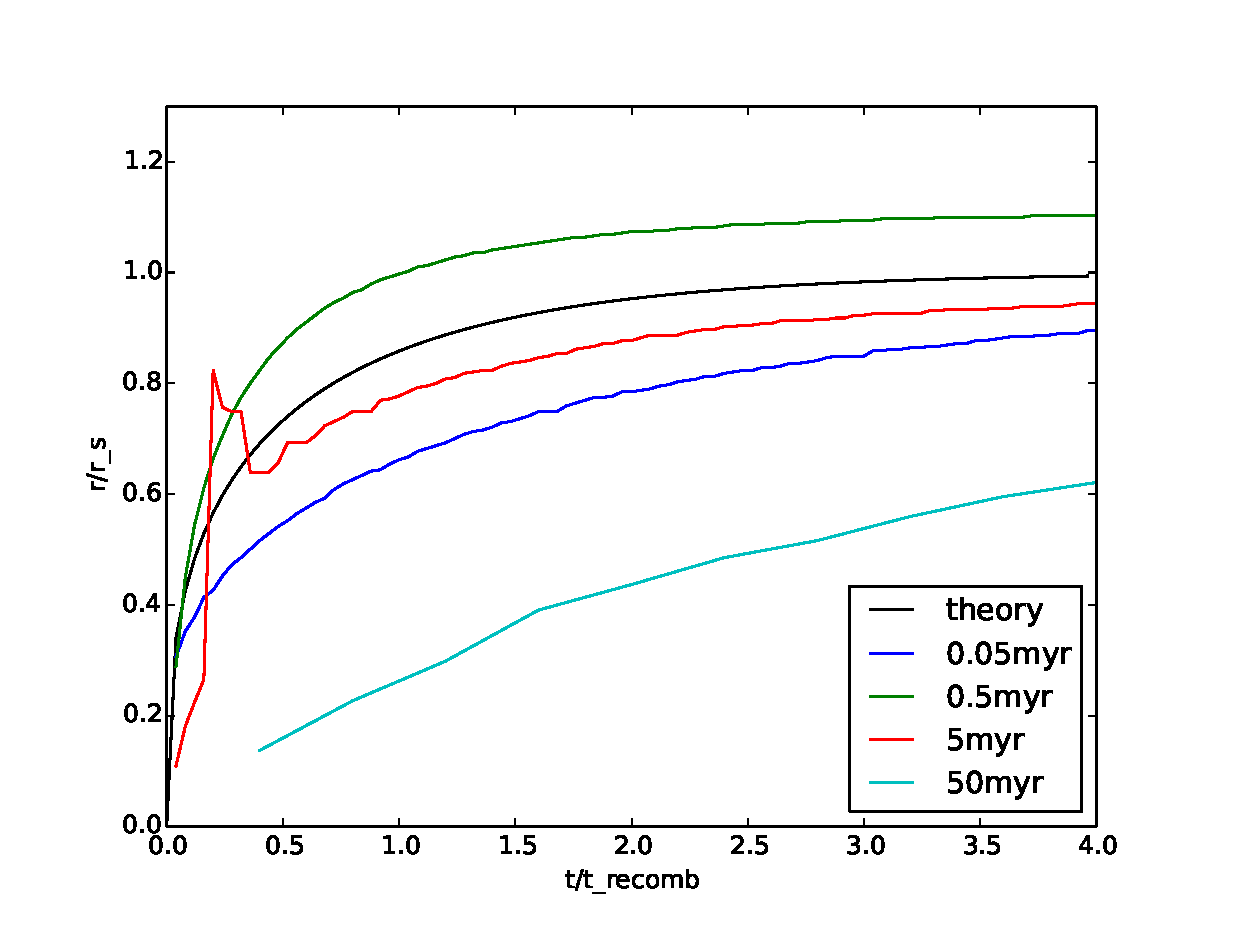
\includegraphics[width=\textwidth]{graphics/rvstime.eps}
\caption[Radius vs time for the isothermal Str\"omgren sphere.]{Radius vs time for the isothermal Str\"omgren sphere test for a number of different time steps.}
\label{fig:stromgrenisorvstime}
\end{figure}

\subsection{The Thermal Case}
\label{sec:thermalstromgren}

The above formulation assumed the gas was isothermal and that all incident photons had the same energy. In reality, photons range across many wavelengths (commonly in a Planck spectrum) with differing cross sections for each wavelength. As well, absorption typically causes heating, which effects, among many properties, recombination rate.

In order to do a more realistic test,the incident photons are assumed to be from a black body with temperature 1e5 K. The cross section is changed to an integrated cross section, obtained by integrating the cross section as a function of wavelength over all wavelengths having energies between 13.6 ev and 29.65 ev. The gas has an initial temperature of 100 K and uses an integrated cross section (over the range of energies present) of $1.63\e{-18}$ cm$^{-2}$. The recombination rate is a function of temperature, set to

\begin{equation}
\label{eq:recombpetkova}
\alpha(T) = 2.59\e{-13}\left(\frac{T}{1\e{4}~K}\right)^{-0.7} cm^{-3} s^{-1},
\end{equation}

\noindent
to match \citet{petkovaSpringel09}. This test includes heating due to absorption and cooling due to recombination $\Lambda_r$, collisional ionization $\Lambda_{ci}$, line cooling $\Lambda_l$, and Bremsstrahlung radiation $\Lambda_B$. The rate are taken from \citet{cen92} in order to match \citet{petkovaSpringel09}. The following are those rates in ergs cm$^{-3}$ s$^{-1}$:

\begin{align}
\label{eq:cencooling}
\Lambda_r & = {8.7\e{-27} \sqrt{T}\left(\frac{T}{10^3 K}\right)^{-0.2}} \Biggm/{\left[1+\left(\frac{T}{10^6 K}\right)^{0.7}\right]}, \\
\Lambda_{ci} & = 1.27\e{21} \sqrt{T}\left(1 + \sqrt{\frac{T}{10^5 K}}\right)e^{157809.1/T} n_e n_{HII},\\
\Lambda_l & = 7.5\e{-19}\left(1+\sqrt{\frac{T}{10^5 K}}\right)^{-1}e^{-118348/T}n_e n_{HI},\\
\Lambda_B & = 1.42\e{-27}g_{ff}\sqrt{T}n_e,
\end{align}

\noindent
where $g_{ff} = 1.3$ is the gaunt factor. This scenario does not have an analytic solution to compare to, and so we instead compare to the results of \citet{ilievEt06} and \citet{petkovaSpringel09}.

\begin{figure}
        \centering
        \begin{subfigure}[b]{0.45\textwidth}
                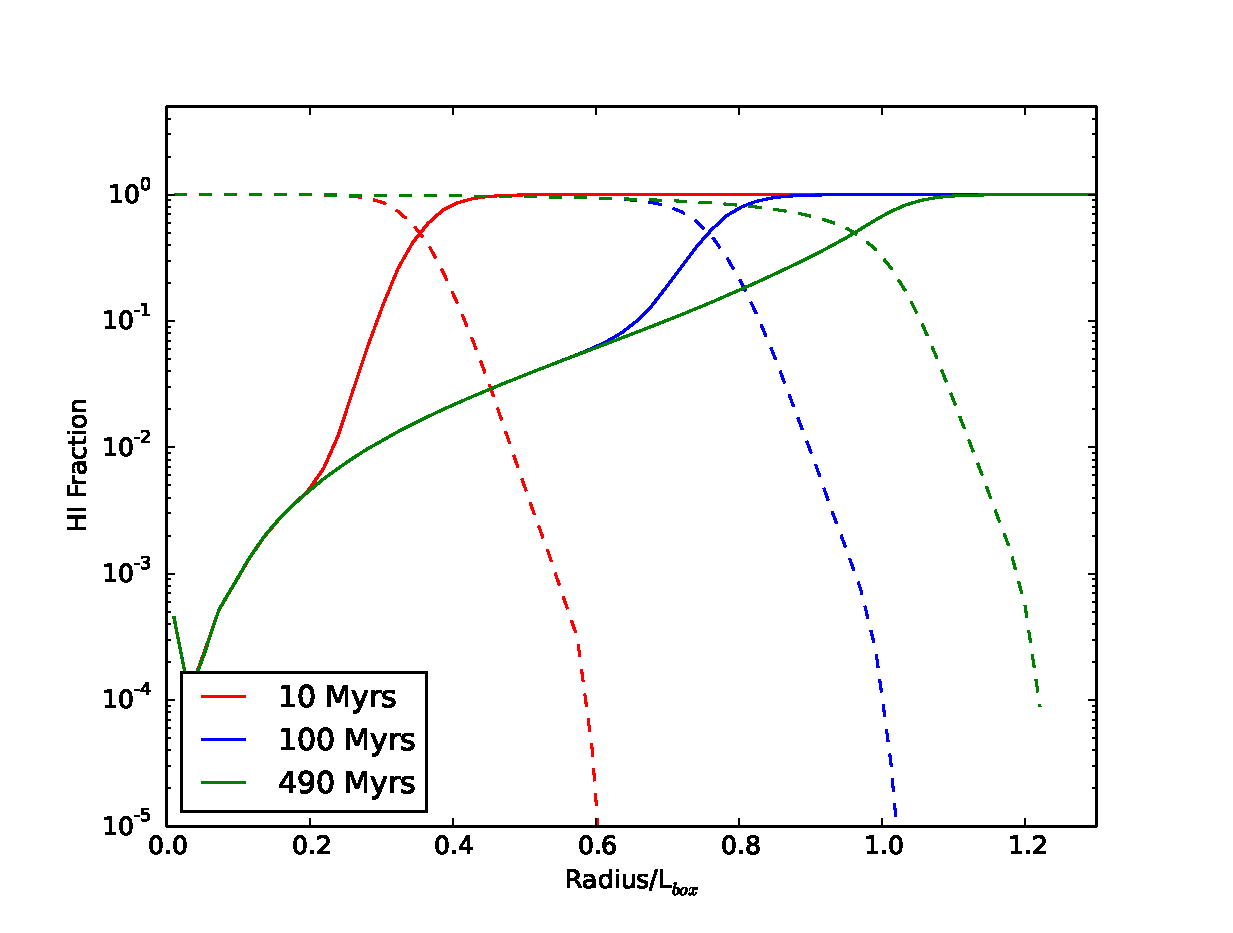
\includegraphics[width=\textwidth]{graphics/HIProfile.eps}
                \caption{}
                \label{fig:stromgrenthermaltemp}
        \end{subfigure}
        ~ 
        \begin{subfigure}[b]{0.45\textwidth}
                \includegraphics[width=\textwidth]{graphics/thermalTempProfile.eps}
                \caption{}
                \label{fig:stromgrenthermalH}
        \end{subfigure}
        \\
        \begin{subfigure}[b]{0.45\textwidth}
                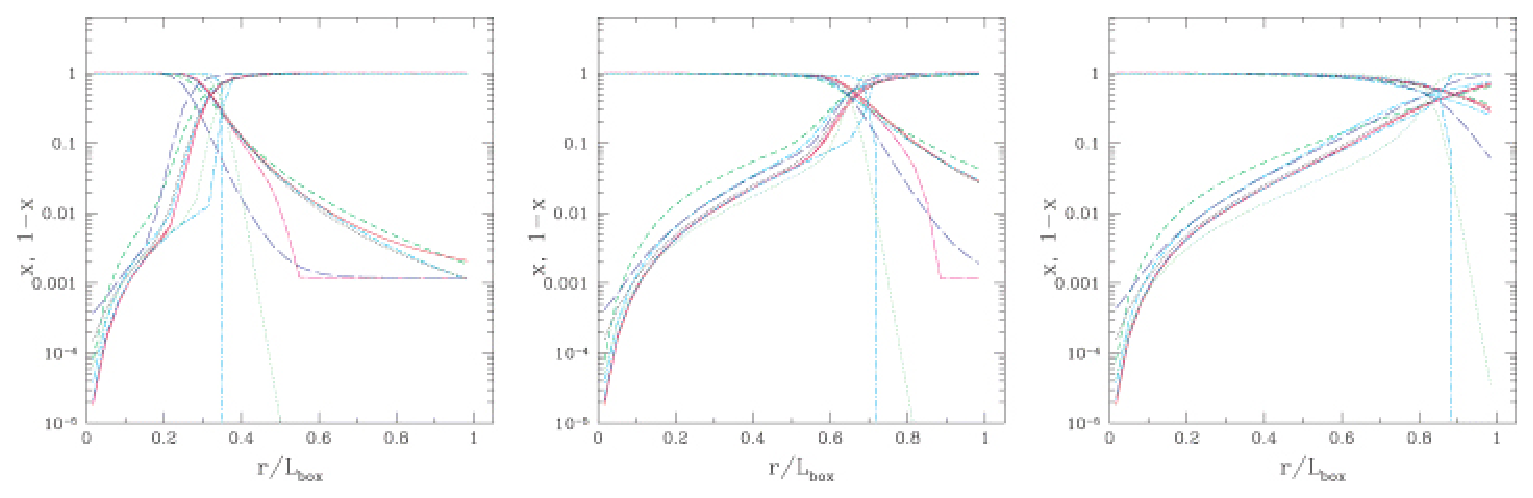
\includegraphics[width=\textwidth]{graphics/iliev06f16.eps}
                \caption{}
                \label{fig:ilievEtf16}
        \end{subfigure}
        ~ 
        \begin{subfigure}[b]{0.45\textwidth}
                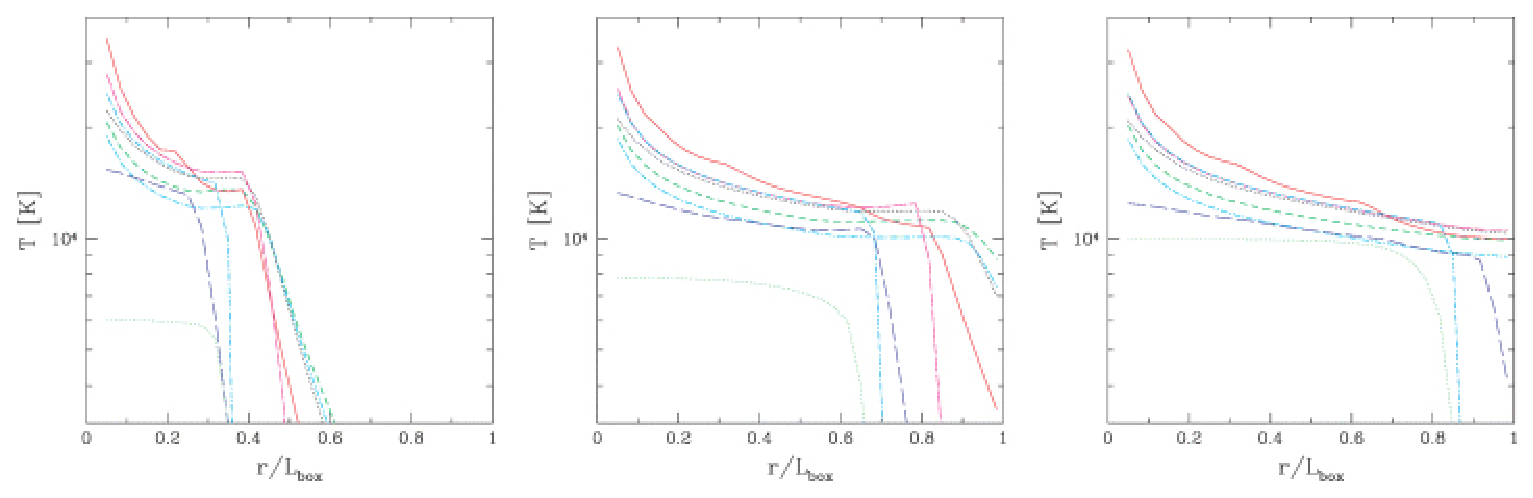
\includegraphics[width=\textwidth]{graphics/iliev06f17.eps}
                \caption{}
                \label{fig:ilievEtf17}
        \end{subfigure}
        \caption[Temperature vs radius and HI vs radius for the thermal Str\"omgren sphere.]{Figure a) shows a temperature profile for the thermal Str\"omgren sphere and figure b) shows the neutral and ionized Hydrogen fraction profiles. The figures are comparable to figures 16 and 17 (c and d above) from \citet{ilievEt06}.}
        \label{fig:stromgrenthermal}
\end{figure}

Figure \ref{fig:stromgrenthermal} shows a radial temperature profile and radial neutral and ionized Hydrogen fraction profile. The figures can be compared directly with figures 16 and 17 from \citet{ilievEt06}. We see a peak temperature of roughly $3\e{4} K$ with a radial dropoff similar to results from \citet{ilievEt06}.

\section{The Blister HII Region}
\label{sec:gaswall}

In order to test the algorithm's ability to handle a sharp density jump, we again perform the isothermal Str\"omgren front (section \ref{sec:isostromgren}), but with a large density jump. We keep all of the same initial parameters, but change the density to the left of x = 0 to $n_0/2$ and the density to the right of x = 0 to $3/2 n_0$, where $n_0$ is 1e-3 cm$^{-3}$. This scenario is similar to a blister HII region where a star is at the edge of a dense cloud. Radiation into the cloud will be much more largely attenuated than radiation outwards from the cloud.

\subsection{Radiation Only}
\label{sec:gaswallradonly}

In the case that hydrodynamics is off, the solution is two str\"omgren hemispheres centered at x = 0. For the lower density on the left, this gives a Str\"omgren radius of 8.54  kpc, and for the higher density on the right, a radius of 4.11 kpc. This gives recombination times of 250 Myr and 83.3 Myr, respectively.

\begin{figure}
		\centering
        \begin{subfigure}[b]{\textwidth}
                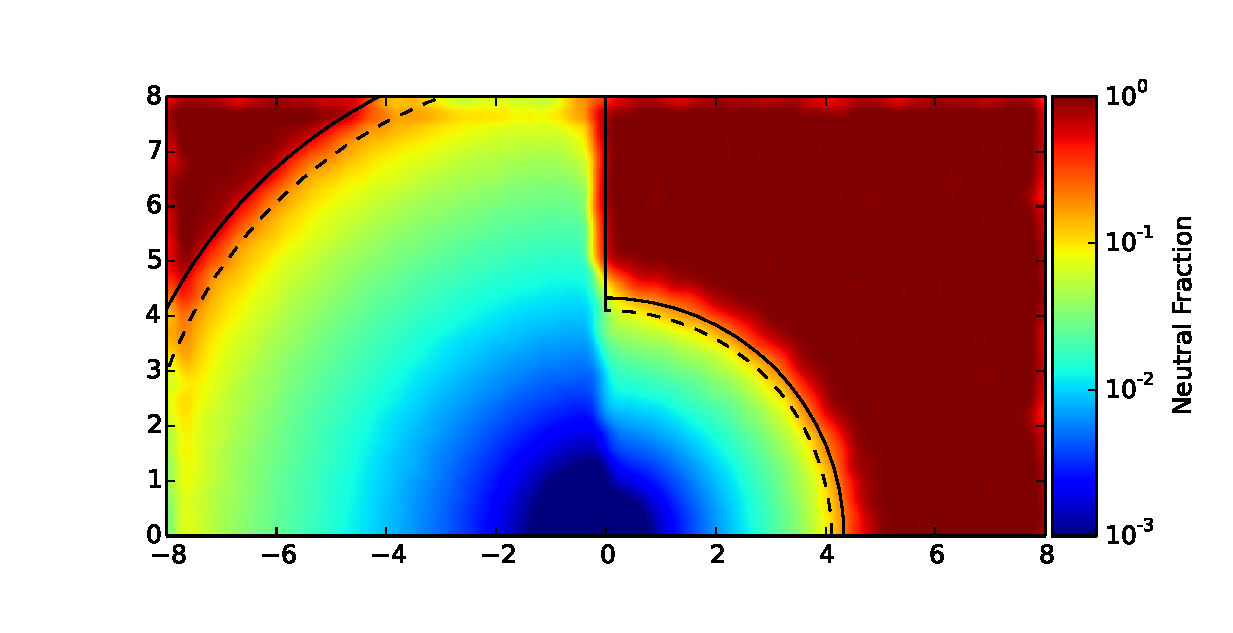
\includegraphics[width=\textwidth]{graphics/gasWall01000slice.eps}
                \caption{}
                \label{fig:gaswallslice}
        \end{subfigure}
        \\
        \begin{subfigure}[b]{\textwidth}
                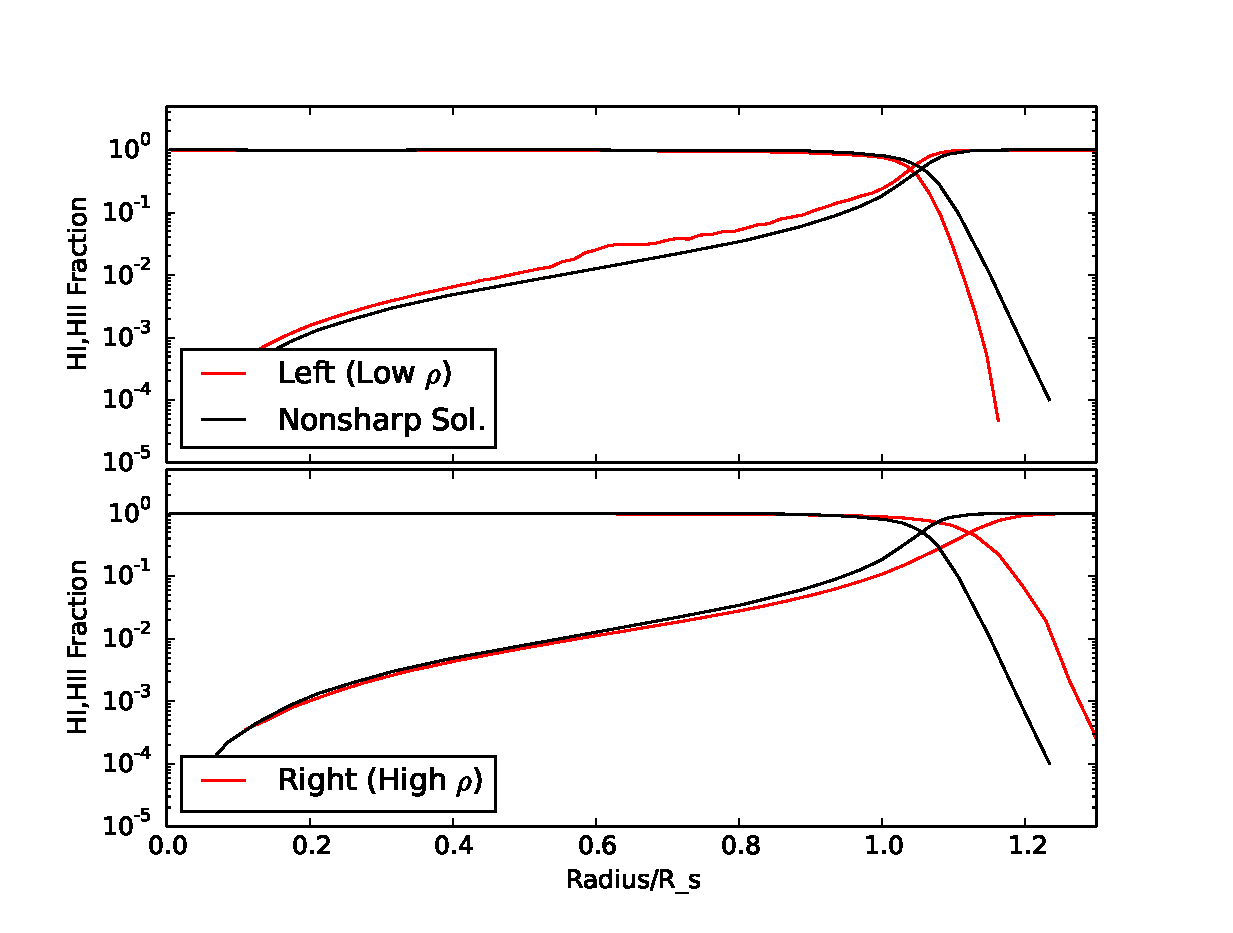
\includegraphics[width=\textwidth]{graphics/gasWall01000HI.eps}
                \caption{}
                \label{fig:gaswallHI}
        \end{subfigure}
	\caption[Blister region without hydrodynamics]{Stuff.}
	\label{fig:gaswall}
\end{figure}

Figure \ref{fig:gaswallslice} shows a slice in the z plane across the simulation. The solid black line is the solution to the non-sharp ionization front, and the dashed line is the sharp ionization front solution. We see the code is able to sharply resolve interface between the high and low density region, producing two Str\"omgren hemispheres of different radii. In the low density region, the ionization front has made it all the way to the edge of the box, so we see some edge effects at the top and left parts of the hemisphere.

Figure \ref{fig:gaswallHI} are radial profiles of HI and HII for each half of the cube, scaled to the calculated sharp Str\"omgren radius. The black line again represents the solution to the non-sharp ionization front. We see that in this case, results are not quite as clean as a homogeneous box. The low density region is under-ionized compared to the non-sharp solution, and the high density region is over-ionized.

The under/over ionization issue is a consequence of using average properties of the sending (luminous) cell. For leaves that are sufficiently far away, an interaction with a cell center of luminosity is accepted. When the tree climb is performed from the sending cell side, the average density is used to get $\tau_i$ ($\tau_i = \rho_i \kappa_i ds$). In the direction of the high density region, the average density is too low since the ray is contained entirely in the high density side and vice versa. While the error is not significant, it is a consequence of the way the algorithm has been developed. Including higher order moments of the luminosity distribution in the sending cells could improve results in situations like this (see chapter \ref{chap:conclusions}).

\subsection{With Hydrodynamics - the Champagne Flow}
\label{sec:champagne}

In order to test the coupling of radiation to the hydrodynamics, we perform a similar test in which the code now uses its hydrodynamics solvers. We follow the setup of \citet{gendelevKrumholz12}; A 50 pc cube is initialized with a density of 0.055 atoms cm$^{-3}$ to the right of x = 0, and 63 atoms cm$^{3}$ to the left. The temperatures of the left and right halves are 55 K and 6.3e3 K, respectively. This density/temperature combination gives pressure equilibrium at the boundary. An ionizing source is turned on at the origin that emits 5.3e47 photons/s, similar to a type BO.5 star. The combination of density and luminosity gives a Str\"omgren radius of 1.5 pc in the dense region and a recombination time of 2.48e4 Years. The simulation is run for 5e6 Myrs.

Timescales of 10$^5$ yrs or longer mean that hydrodynamics now have sufficient time to act on the gas. \citet{spitzer78} shows that the expansion of a shell of gas around an HII region due to heating is described as

\begin{equation}
\label{eq:spitzerexpansion}
R_{sh} = R_s\left(1 + \frac{7t}{4t_s}\right)^{4/7},
\end{equation}

\noindent
where $R_{sh}$ is the radius of the expanding shell, $R_s$ is the Str\"omgren radius, t is the time since radiation started, and $t_s = r_s/cII$, where $cII$ is the sound speed in the ionized region. \citet{hosawaInutsuka06} Derive a similar relationship, but include an extra factor of $\sqrt{4/3}$

\begin{equation}
\label{eq:hosawaexpansion}
R_{sh} = R_s\left(1 + \sqrt{\frac{4}{3}}\frac{7t}{sqrt{4}t_s}\right)^{4/7},
\end{equation}

\noindent
which accounts for [WHAT?]. \citet{gendelevKrumholz12} derive the same result, but for a blister region, which differs by a factor of 2 from equation \ref{eq:hosawaexpansion} to account for [WHAT?],

\begin{equation}
\label{eq:spitzerexpansion}
R_{sh} = R_s\left(\frac{7t}{\sqrt{6}t_s}\right)^{4/7}.
\end{equation}

\begin{figure}
        \centering
        \begin{subfigure}[b]{0.3\textwidth}
                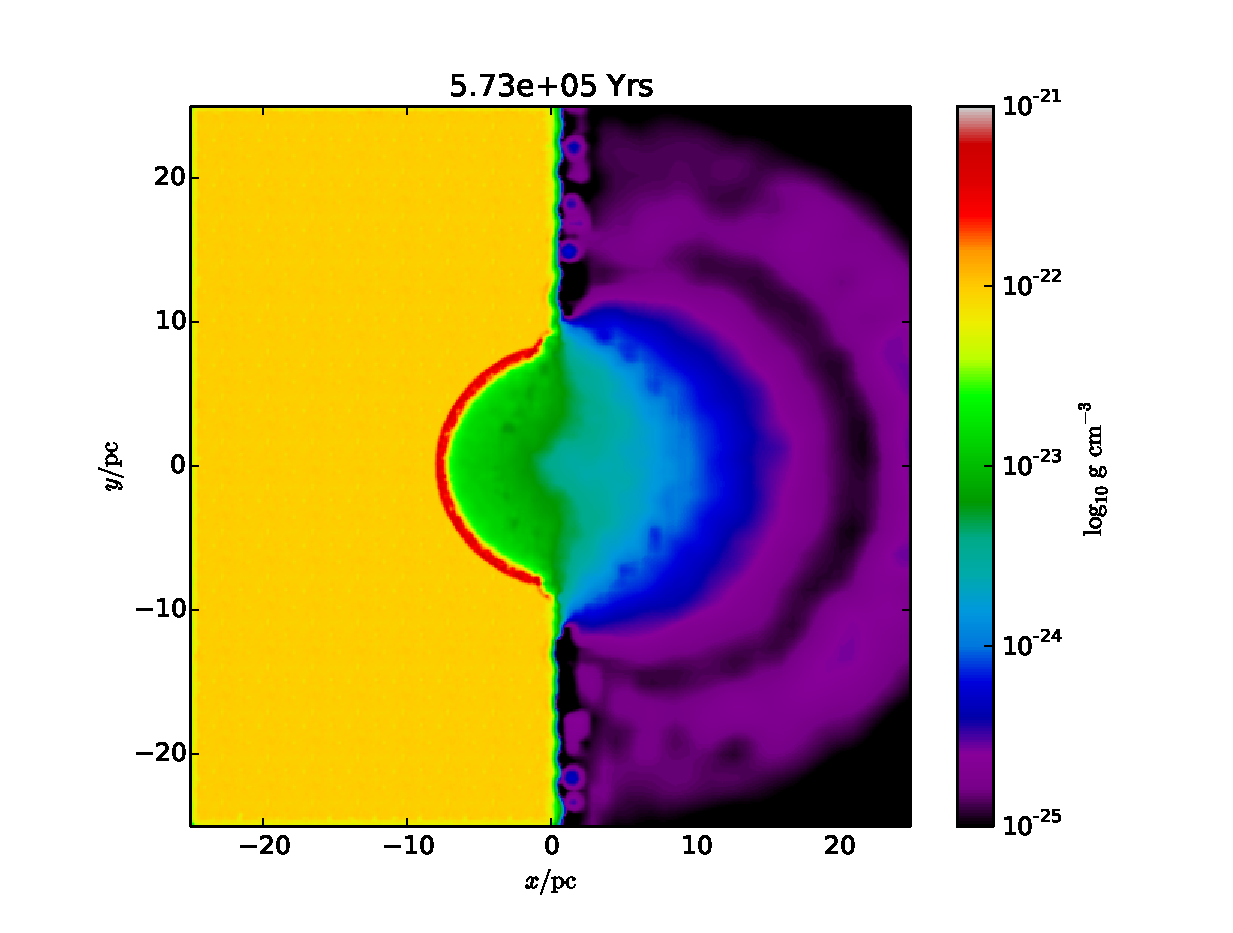
\includegraphics[width=\textwidth]{graphics/blister25600040rhoslice.eps}
                \caption{0.5 Myr}
                \label{fig:champagne1}
        \end{subfigure}
        ~ 
        \begin{subfigure}[b]{0.3\textwidth}
                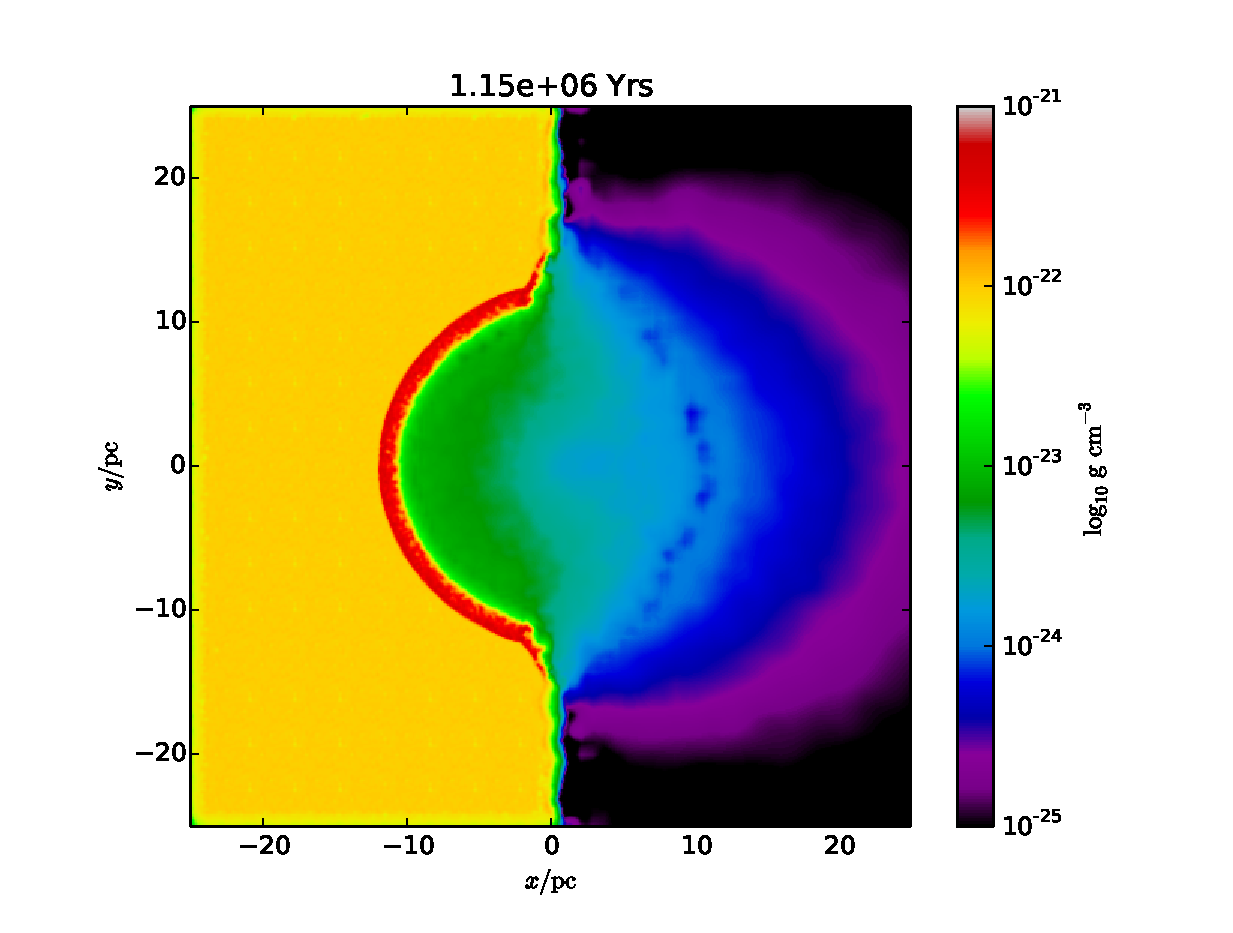
\includegraphics[width=\textwidth]{graphics/blister25600080rhoslice.eps}
                \caption{1 Myr}
                \label{fig:champagne2}
        \end{subfigure}
         ~ 
        \begin{subfigure}[b]{0.3\textwidth}
                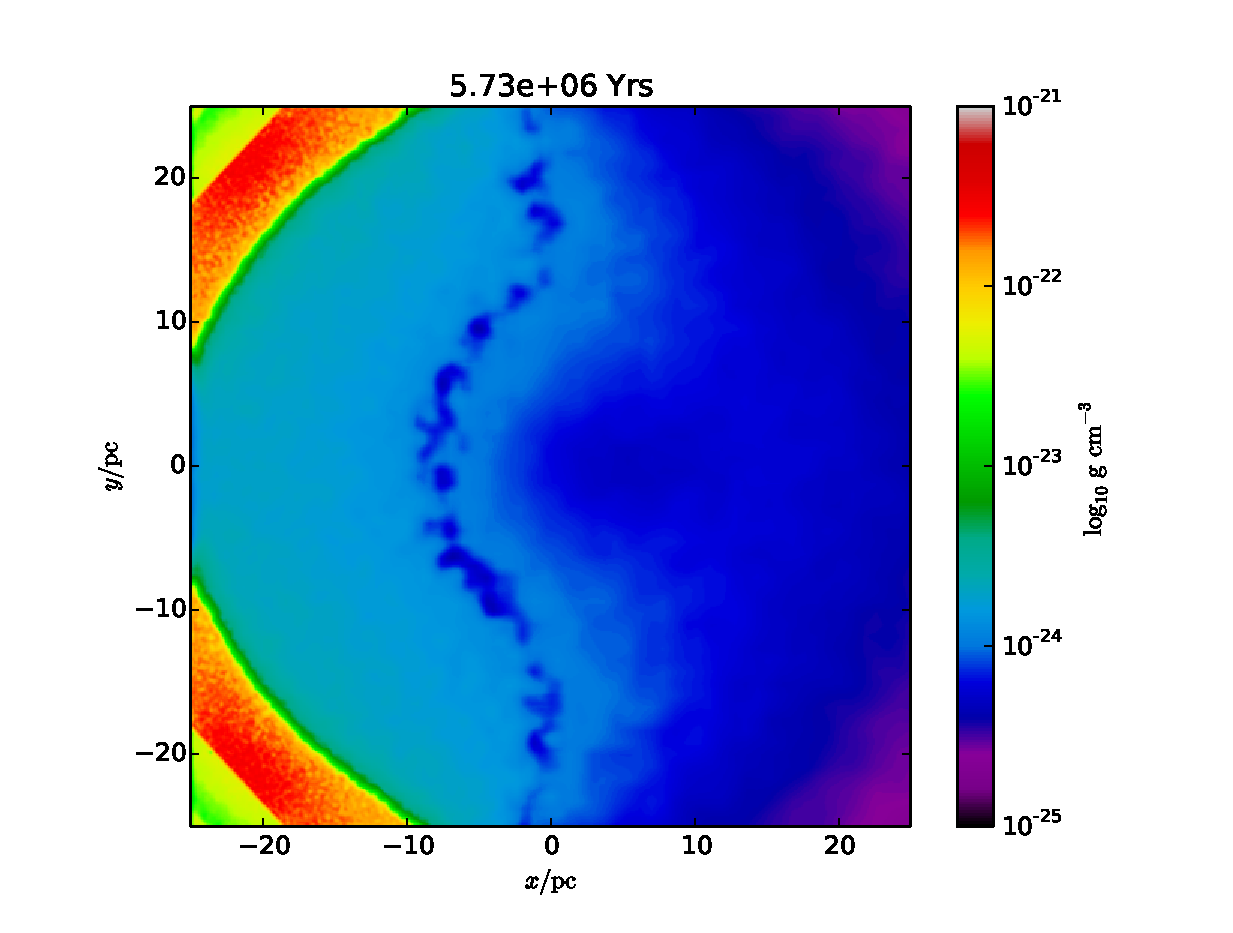
\includegraphics[width=\textwidth]{graphics/blister25600400rhoslice.eps}
                \caption{5 Myrs}
                \label{fig:champagne3}
        \end{subfigure}
        \caption[A champagne flow.]{The Blister HII region from \citet{gendelevKrumholz12}.}
        \label{fig:champagne}
\end{figure}

\section{Shadowing}
\label{sec:shadowing}

\subsection{Simple Shadow Test}
\label{sec:simpleshadow}

We present the shadowing test from \citet{hayesNorman03,gonzalezEt07,skinnerOstriker13}. A thin 2-D tube of gas with dimensions 0.12 cm tall x 1 cm long is irradiated from the left by a distant ((x,y) = (-100,0) cm) source with a characteristic temperature of 1740 K. The gas has an ambient density of $\rho_0 = 0.001 g cm^{-3}$ and an ambient temperature of 290 K. An oblate spheroid with dimensions $(x_0,y_0) = (0.1,0.06)$ cm is placed in the tube at $(x_c,y_c) = (0.5,0)$ cm. The spheroid has a central density of $\rho_1 = 1000\rho_0 = 1$ g~cm$^{-3}$ and the same ambient temperature. Note that hydrodynamics is turned off, so a mismatch in pressure is not an issue. The cloud has a density structure described by

\begin{equation}
\label{eq:shadowdensity}
\rho_{cloud}(x,y) = \rho_0 + \frac{(\rho_1 - \rho_0)}{(1+e^{\Delta})},
\end{equation}

\noindent
where

\begin{equation}
\label{eq:shadowdelta}
\Delta = 10\left\lbrace\left[\frac{x-x_c)}{x_0}\right]^2 + \left[\frac{y-y_c}{y_0}\right]^2-1\right\rbrace.
\end{equation}

This structure gives the cloud a ``fuzzy'' surface in that the density smoothly transitions rather than sharply jumps. The opacity is set as a function of density and temperature,

\begin{equation}
\label{eq:shadowopacity}
\kappa(T_{gas},\rho) = \kappa_0\left(\frac{T_{gas}}{T_0}\right)^{-3.5}\left(\frac{\rho}{\rho_0}\right),
\end{equation}

\noindent
with $\kappa_0 = 100$~cm$^2$~g$^{-1}$. This gives an optical depth of 0.1 across the length of the box, excluding the dense cloud, and an optical depth of roughly 2000 across the diameter of the blob.

The tube is resolved by 280x80 SPH resolution elements, and the above density structure is obtained by changing the mass of the SPH particles (as opposed to increasing the number of particles). Note that this is not realistic for SPH, where higher densities are usually represented by a higher density of particles. However, we have elected to keep the same resolution as previous papers to aid in comparison.

At t = 0, the source is turned on and the simulation is evolved for 0.1 s, or $3\e{9}$ light crossing times. Figure \ref{fig:shadow} shows the simulation at t = 0.1 s.

\begin{figure}
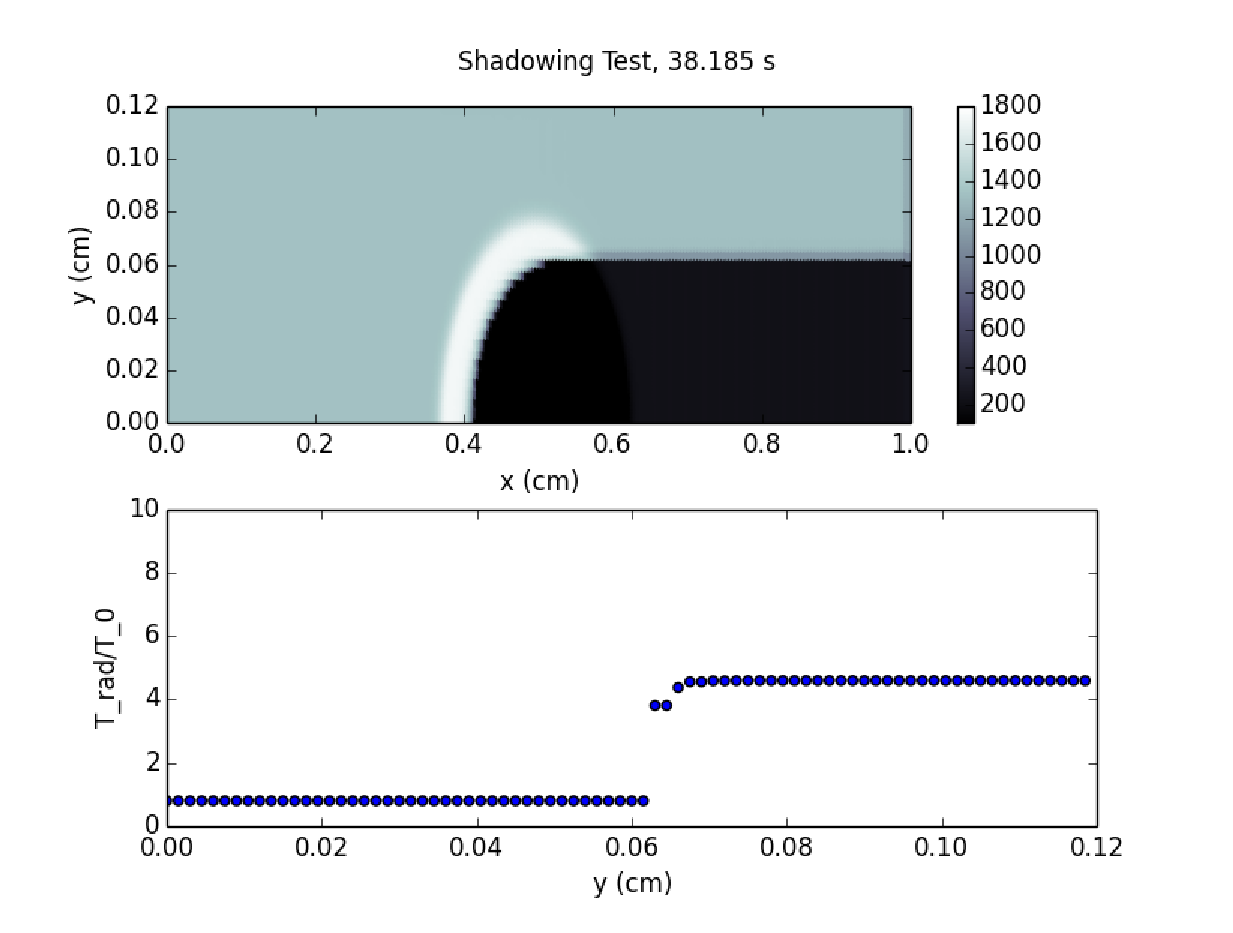
\includegraphics[width=\textwidth]{graphics/shadow10000.eps}
\caption[Shadowing behind a dense clump.]{A shadow created behind a dense ellipsoid of gas. The top frame is a plot of radiation temperature, and the bottom frame is a vertical temperature profile at the right edge of the box.}
\label{fig:shadow}
\end{figure}

Figure \ref{fig:shadow} shows the radiation temperature

\begin{equation}
\label{eq:radtemp}
T_{rad} = T_0 \left(\frac{F_0}{F_f}\right)^{1/4},
\end{equation}

\noindent
Where $T_0$ is the initial temperature of the radiation (290 K), $F_0$ is the initial flux at the left edge, and $F_f$ is the final flux at any position.

We see a sharp shadow cast behind the blob, with no signs of diffusion. Ray tracing methods create excellent shadows, so it is unsurprising that our method, which uses reverse ray tracing, creates a good shadow as well.


\subsection{Ionization Front Trapping}
\label{sec:ifronttrapping}

Along the same lines of section \ref{sec:simpleshadow}, this section performs a shadowing test. However, this test includes ionizing radiation and is constructed in such a way that the ionization front should stall out inside of the dense sphere. The test is taken from \citet{ilievEt06}.

A 6.6 kpc cube is initiated with mean background density $2\e{-4} cm^{-3}$ and background temperature 8000 K. The dense clump is located at (x,y,z) = (5,3.3,3.3) and is given a density of 200 times the background, or 0.04 $cm^{-3}$, and a temperature of 40 K.

The conditions for trapping an ionization front are presented in \citet{shapiroEt04}. The authors show that a clump can trap an ionization front if

\begin{equation}
\label{eq:ifronttrap}
l_s = \frac{F}{\alpha n_H^2}
\end{equation}

\noindent
is less than the diameter of the clump, where $F$ is the flux in photons s$^{-1}$. In the above simulation $\alpha = 2.59\e{-13} (T/10^4 K)^{-3/4}$, which at a temperature of $10^4$ K, the clump should trap the ionization front about 0.78 kpc, or just about halfway into the clump. The estimate is rough, particularly for SPH, due to the variation in temperature (and thus the variation in the recombination rate) and the variation in the density field of the clump. We note that due to the nature of SPH, it is very difficult to create a clump with so few particles that has a sharp density jump compared to the size of the clump.

\begin{figure}
        \centering
        \begin{subfigure}[b]{0.45\textwidth}
                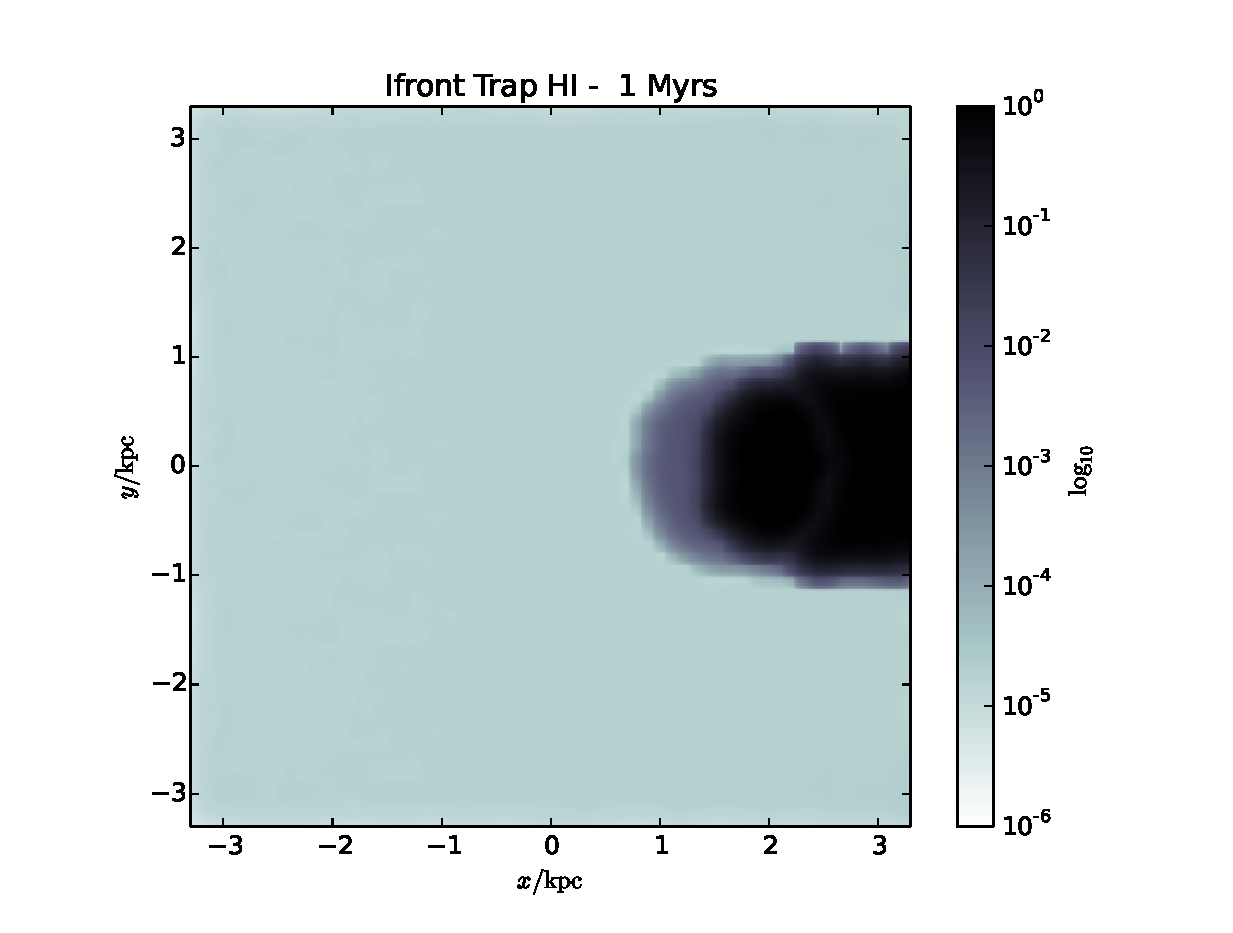
\includegraphics[width=\textwidth]{graphics/ifrontTrap00010HI.eps}
                \caption{HI, 1 Myr}
                \label{fig:ifronttrap1a}
        \end{subfigure}
        ~ 
        \begin{subfigure}[b]{0.45\textwidth}
                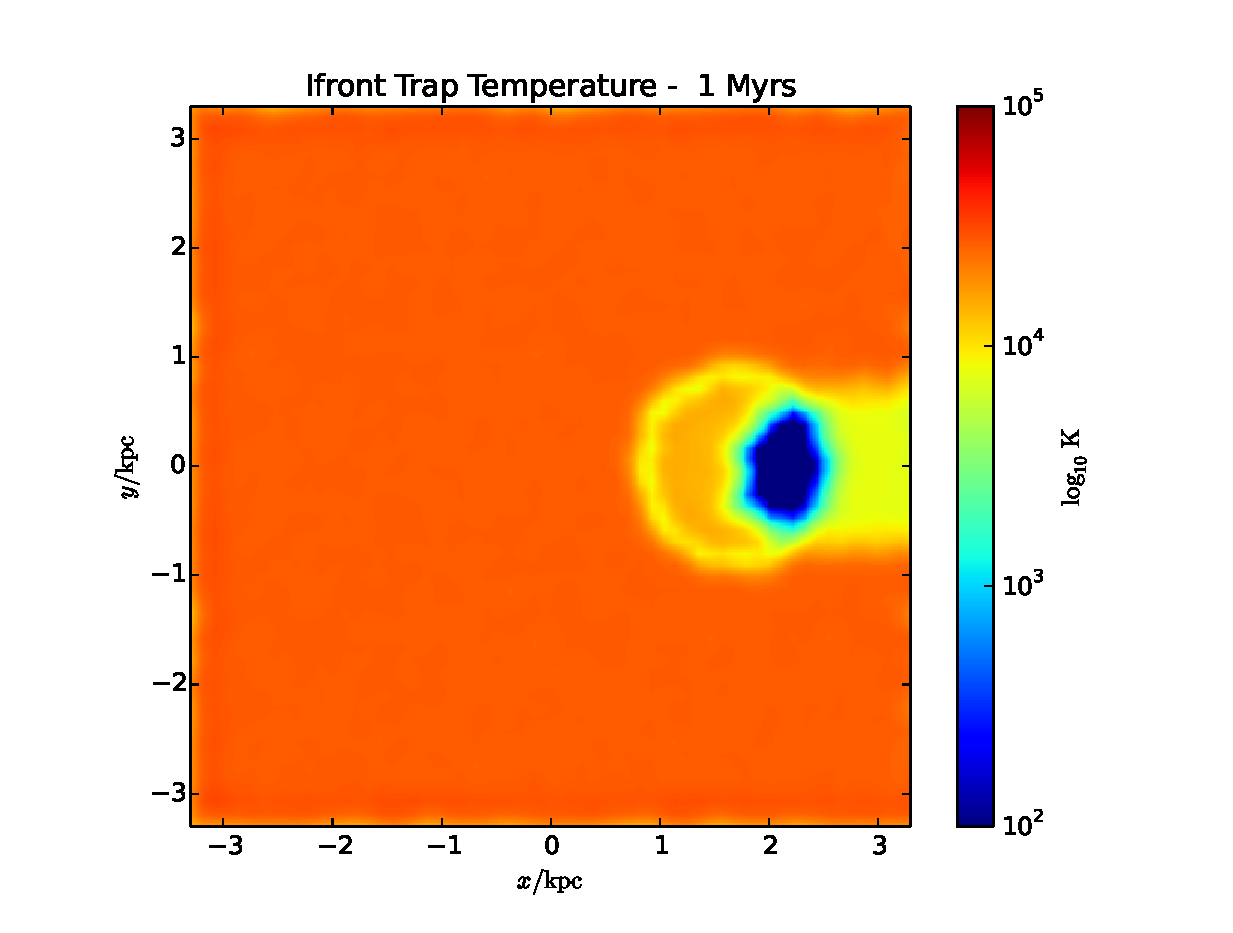
\includegraphics[width=\textwidth]{graphics/ifrontTrap00010Temp.eps}
                \caption{T, 1 Myr}
                \label{fig:ifronttrap1b}
        \end{subfigure}
        \\
        \begin{subfigure}[b]{0.45\textwidth}
                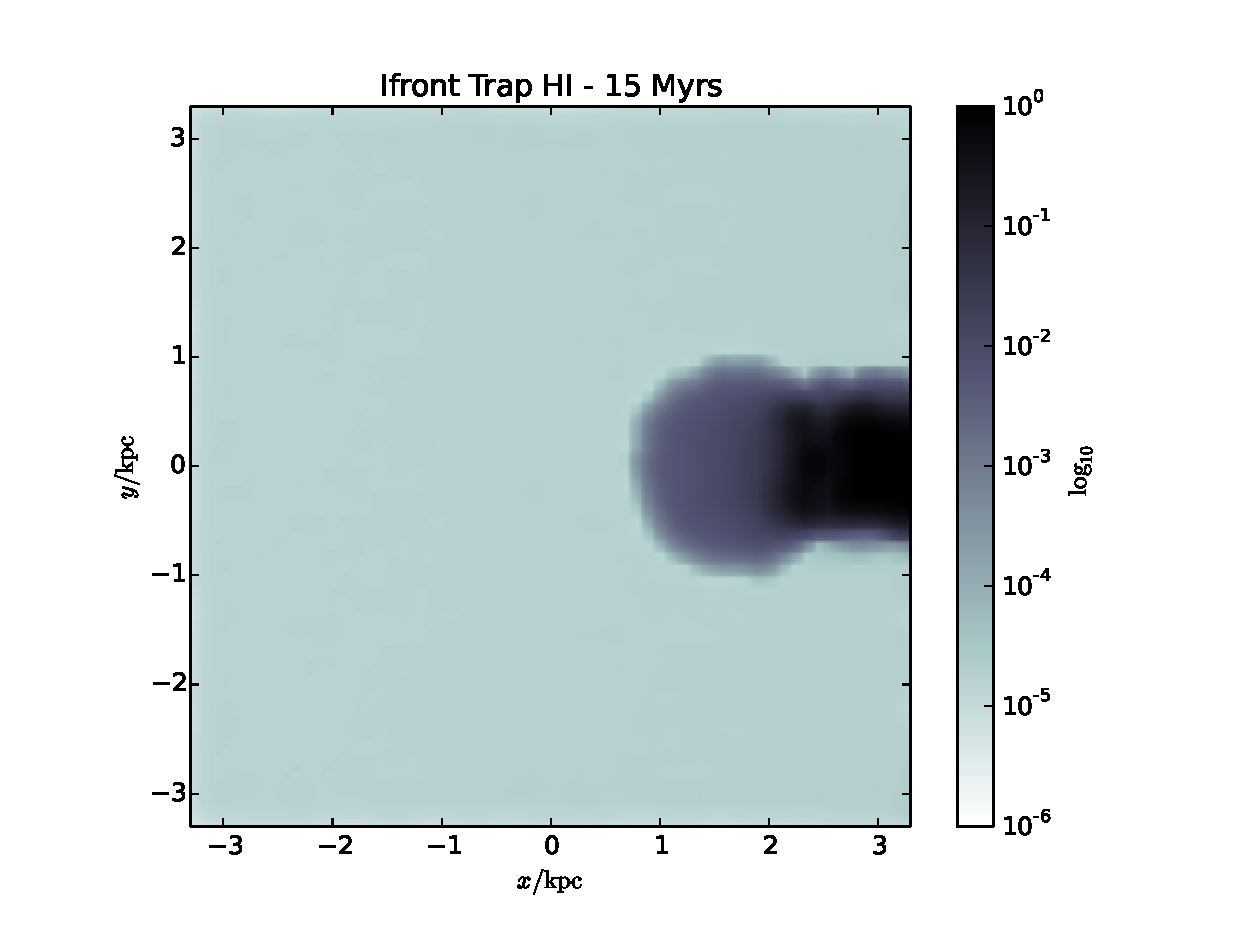
\includegraphics[width=\textwidth]{graphics/ifrontTrap00150HI.eps}
                \caption{HI, 15 Myrs}
                \label{fig:ifronttrap15a}
        \end{subfigure}
        ~ 
        \begin{subfigure}[b]{0.45\textwidth}
                \includegraphics[width=\textwidth]{graphics/ifrontTrap00150Temp.eps}
                \caption{T, 15 Myrs}
                \label{fig:ifronttrap15b}
        \end{subfigure}
        \caption[Ionization front trapping.]{}
        \label{fig:ifronttrap}
\end{figure}

Figure\ref{fig:ifronttrap} shows the simulation at time t = 1 Myr and t = 15 Myr. The left column (\ref{fig:ifronttrap1a} and \ref{fig:ifronttrap15a}) show a slice in the Z plane of HI fraction. The right column (\ref{fig:ifronttrap15a} and \ref{fig:ifronttrap15b}) show a slice in the Z plane of temperature. These figures are comparable to figures 22-25 of \citet{ilievEt06}. The ionization front makes it significantly further through the sphere in our runs compared to most of the runs from \citet{ilievEt06}.

\begin{figure}
\includegraphics[width = \textwidth]{graphics/timeseries.eps}
\caption[HII and Temperature vs time.]{Average Ionization fraction and temperature inside the sphere vs time.}
\end{figure}

In order to see why we over-ionize our sphere, we look at a time series of the average ionization fraction and temperature in our sphere. This plot is comparable to figure 26 from \citet{ilievEt06}. We see that we tend to overheat the gas, which leads to a lower recombination rate. Our run equilibrates at about 1.4e4 K, compared to about 1.1e4 K for most runs from \citet{ilievEt06}. This creates a change in recombination rate of about 26\%, which changes the trapping distance (equation \ref{eq:ifronttrap}) to roughly 1 kpc, or 5/8 of the way through the sphere.

The IC that was created for this test contains only 470 particles inside of the dense sphere, which is roughly 8 particles across. For this reason, the density of the sphere has a radial dropoff in density from the target density of roughly 0.04 cm$^-3$ to 0.03 cm$^{-3}$. A 25\% change in density could account for the discrepancies seen in the above figures. Keep in mind that if a similar situation appeared in a simulation, the results would be improved due to a higher effective resolution in the dense clump.

